\begin{frame}
  \frametitle{Feature Interaction - Motivation}
  \begin{itemize}
  \item Is Feature Effect a good approach?
    \begin{itemize}
    \item Interpretability $\rightarrow$ very good, easy intuition
    \item Fidelity $\rightarrow$ it depends..
    \end{itemize}
  \item Additive case: \(f(\xb) = f_1(x_1) + f_2(x_2)\)
    \begin{itemize}
    \item Generalized Additive Models
      \item X-by-design
    \end{itemize}

\item Non-additive case: \(f(\xb) = f_1(x_1) + f_2(x_2) + \underbrace{f_{12}(x_1, x_2)}_{interaction}\)
  \begin{itemize}
  \item how to distribute \(f_{12}(x_1, x_2)\) to \(x_1\) and \(x_2\)?
  \item Research question; uncertainty could help
  \end{itemize}
  \item \(f\) is unknown,
  \item what is the magnitude of the interaction terms?
  \item Feature Interaction methods!
\end{itemize}
\end{frame}


\begin{frame}
  \frametitle{Problem Statement}
  When features interact with each other in a prediction model, the prediction cannot be expressed as the sum of the feature effects, because the effect of one feature depends on the value of the other feature. Aristotle’s predicate “The whole is greater than the sum of its parts” applies in the presence of interactions.\footnote{\href{https://christophm.github.io/interpretable-ml-book/interaction.html}{Interpretable Machine Learning book}}
\end{frame}


\begin{frame}
  \frametitle{H-statistic}
  \begin{itemize}
  \item Level of interaction between feature \(i\) and feature \(j\)
  \end{itemize}

  \[ \mathcal{H}^2_{jk} = \frac{\sum_{i=1}^n \left ( PD_{jk}(x^{(i)}_j, x^{(i)}_k) - PD_{j}(x^{(i)}_j) - PD_{k}(x^{(i)}_k)\right )^2 }{\sum_{i=1}^n PD^2_{jk}(x^{(i)}_j, x^{(i)}_k) } \]

  \begin{itemize}
  \item Level of interaction between feature \(i\) and all the other features
  \end{itemize}

    \[ \mathcal{H}^2_{j} = \frac{\sum_{i=1}^n \left ( f(x^{(i)}) - PD_{j}(x^{(i)}_j) - PD_{-j}(x^{(i)}_{-j})\right )^2 }{\sum_{i=1}^n f^2(x^{(i)}) } \]


\end{frame}


\begin{frame}
  \frametitle{H-statistic}
   \begin{figure}
     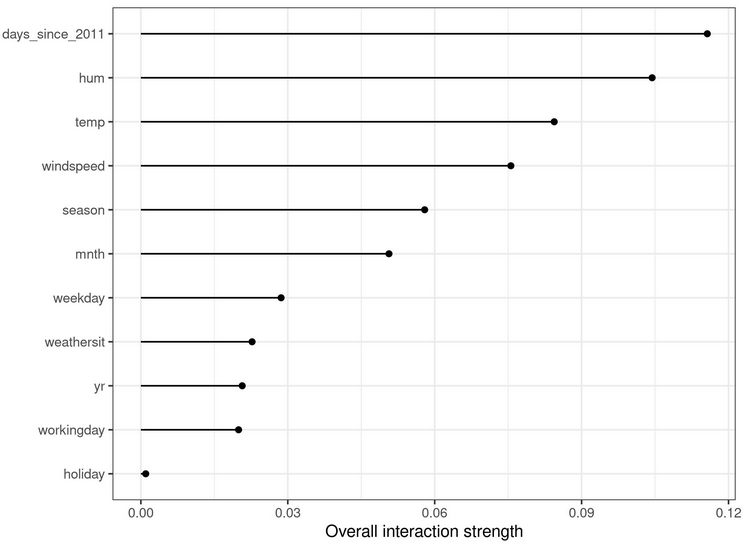
\includegraphics[width=0.8\textwidth]{h_statistic}
     \caption{\footnotesize C. Molnar, IML book}
   \end{figure}

\end{frame}


\begin{frame}
  \frametitle{Other approaches}
  \begin{itemize}
  \item Greenwell's interaction index
    \begin{itemize}
    \item PDP-based method
      \item \href{https://arxiv.org/pdf/1805.04755.pdf}{A Simple and Effective Model-Based Variable Importance Measure}
    \end{itemize}
  \item SHAP interaction index
    \begin{itemize}
    \item SHAP-based method
    \item \href{https://arxiv.org/abs/1802.03888}{Consistent Individualized Feature Attribution for Tree Ensembles}
    \end{itemize}
  \end{itemize}
\end{frame}
